\documentclass[twoside]{book}

% Packages required by doxygen
\usepackage{fixltx2e}
\usepackage{calc}
\usepackage{doxygen}
\usepackage{graphicx}
\usepackage[utf8]{inputenc}
\usepackage{makeidx}
\usepackage{multicol}
\usepackage{multirow}
\PassOptionsToPackage{warn}{textcomp}
\usepackage{textcomp}
\usepackage[nointegrals]{wasysym}
\usepackage[table]{xcolor}

% Font selection
\usepackage[T1]{fontenc}
\usepackage{mathptmx}
\usepackage[scaled=.90]{helvet}
\usepackage{courier}
\usepackage{amssymb}
\usepackage{sectsty}
\renewcommand{\familydefault}{\sfdefault}
\allsectionsfont{%
  \fontseries{bc}\selectfont%
  \color{darkgray}%
}
\renewcommand{\DoxyLabelFont}{%
  \fontseries{bc}\selectfont%
  \color{darkgray}%
}
\newcommand{\+}{\discretionary{\mbox{\scriptsize$\hookleftarrow$}}{}{}}

% Page & text layout
\usepackage{geometry}
\geometry{%
  a4paper,%
  top=2.5cm,%
  bottom=2.5cm,%
  left=2.5cm,%
  right=2.5cm%
}
\tolerance=750
\hfuzz=15pt
\hbadness=750
\setlength{\emergencystretch}{15pt}
\setlength{\parindent}{0cm}
\setlength{\parskip}{0.2cm}
\makeatletter
\renewcommand{\paragraph}{%
  \@startsection{paragraph}{4}{0ex}{-1.0ex}{1.0ex}{%
    \normalfont\normalsize\bfseries\SS@parafont%
  }%
}
\renewcommand{\subparagraph}{%
  \@startsection{subparagraph}{5}{0ex}{-1.0ex}{1.0ex}{%
    \normalfont\normalsize\bfseries\SS@subparafont%
  }%
}
\makeatother

% Headers & footers
\usepackage{fancyhdr}
\pagestyle{fancyplain}
\fancyhead[LE]{\fancyplain{}{\bfseries\thepage}}
\fancyhead[CE]{\fancyplain{}{}}
\fancyhead[RE]{\fancyplain{}{\bfseries\leftmark}}
\fancyhead[LO]{\fancyplain{}{\bfseries\rightmark}}
\fancyhead[CO]{\fancyplain{}{}}
\fancyhead[RO]{\fancyplain{}{\bfseries\thepage}}
\fancyfoot[LE]{\fancyplain{}{}}
\fancyfoot[CE]{\fancyplain{}{}}
\fancyfoot[RE]{\fancyplain{}{\bfseries\scriptsize Generated on Wed Apr 6 2016 10\+:48\+:54 for Velocity Determination of a Quad-\/\+Rotor U\+A\+V by Doxygen }}
\fancyfoot[LO]{\fancyplain{}{\bfseries\scriptsize Generated on Wed Apr 6 2016 10\+:48\+:54 for Velocity Determination of a Quad-\/\+Rotor U\+A\+V by Doxygen }}
\fancyfoot[CO]{\fancyplain{}{}}
\fancyfoot[RO]{\fancyplain{}{}}
\renewcommand{\footrulewidth}{0.4pt}
\renewcommand{\chaptermark}[1]{%
  \markboth{#1}{}%
}
\renewcommand{\sectionmark}[1]{%
  \markright{\thesection\ #1}%
}

% Indices & bibliography
\usepackage{natbib}
\usepackage[titles]{tocloft}
\setcounter{tocdepth}{3}
\setcounter{secnumdepth}{5}
\makeindex

% Hyperlinks (required, but should be loaded last)
\usepackage{ifpdf}
\ifpdf
  \usepackage[pdftex,pagebackref=true]{hyperref}
\else
  \usepackage[ps2pdf,pagebackref=true]{hyperref}
\fi
\hypersetup{%
  colorlinks=true,%
  linkcolor=blue,%
  citecolor=blue,%
  unicode%
}

% Custom commands
\newcommand{\clearemptydoublepage}{%
  \newpage{\pagestyle{empty}\cleardoublepage}%
}


%===== C O N T E N T S =====

\begin{document}

% Titlepage & ToC
\hypersetup{pageanchor=false,
             bookmarks=true,
             bookmarksnumbered=true,
             pdfencoding=unicode
            }
\pagenumbering{roman}
\begin{titlepage}
\vspace*{7cm}
\begin{center}%
{\Large Velocity Determination of a Quad-\/\+Rotor U\+A\+V \\[1ex]\large Software Manual }\\
\vspace*{1cm}
{\large Generated by Doxygen 1.8.8}\\
\vspace*{0.5cm}
{\small Wed Apr 6 2016 10:48:54}\\
\end{center}
\end{titlepage}
\clearemptydoublepage
\tableofcontents
\clearemptydoublepage
\pagenumbering{arabic}
\hypersetup{pageanchor=true}

%--- Begin generated contents ---
\chapter{Hierarchical Index}
\section{Class Hierarchy}
This inheritance list is sorted roughly, but not completely, alphabetically\+:\begin{DoxyCompactList}
\item \contentsline{section}{Timed\+Data}{\pageref{classTimedData}}{}
\begin{DoxyCompactList}
\item \contentsline{section}{Height}{\pageref{classHeight}}{}
\end{DoxyCompactList}
\item \contentsline{section}{Vertical\+Data}{\pageref{classVerticalData}}{}
\end{DoxyCompactList}

\chapter{Class Index}
\section{Data Structures}
Here are the data structures with brief descriptions\+:\begin{DoxyCompactList}
\item\contentsline{section}{\hyperlink{classHeight}{Height} }{\pageref{classHeight}}{}
\item\contentsline{section}{\hyperlink{classTimedData}{Timed\+Data} }{\pageref{classTimedData}}{}
\item\contentsline{section}{\hyperlink{classVerticalData}{Vertical\+Data} \\*Store two \hyperlink{classHeight}{Height} objects and calculate vertical velocity }{\pageref{classVerticalData}}{}
\end{DoxyCompactList}

\chapter{File Index}
\section{File List}
Here is a list of all documented files with brief descriptions\+:\begin{DoxyCompactList}
\item\contentsline{section}{\hyperlink{mega__sensor_8h}{mega\+\_\+sensor.\+h} \\*Get sensor data }{\pageref{mega__sensor_8h}}{}
\item\contentsline{section}{\hyperlink{velocityCalculate_8hpp}{velocity\+Calculate.\+hpp} \\*Calculate the Horizontal Velocity of a U\+A\+V }{\pageref{velocityCalculate_8hpp}}{}
\item\contentsline{section}{\hyperlink{velocityTracking_8cpp}{velocity\+Tracking.\+cpp} \\*The main program, stores data and calculates velocities }{\pageref{velocityTracking_8cpp}}{}
\end{DoxyCompactList}

\chapter{Class Documentation}
\hypertarget{classHeight}{\section{Height Class Reference}
\label{classHeight}\index{Height@{Height}}
}


Store height data and timestamp.  




{\ttfamily \#include $<$Height.\+hpp$>$}

\subsection*{Public Member Functions}
\begin{DoxyCompactItemize}
\item 
\hyperlink{classHeight_a7fecf5018a116f8234513b222bae6a2f}{Height} ()
\item 
\hyperlink{classHeight_a1e48b1093e67413d817eae7acf1064ad}{Height} (float height, time\+\_\+ttime)
\item 
float \hyperlink{classHeight_a595e201f356217323516c6465f697ca4}{get\+Height} ()
\item 
time\+\_\+t \hyperlink{classHeight_a40db46d3736f83f914a59050abfca92d}{get\+Time} ()
\item 
void \hyperlink{classHeight_afa56baac0be90a36def98b7a5a40788f}{print\+All} ()
\end{DoxyCompactItemize}


\subsection{Detailed Description}
Store height data and timestamp. 



\subsection{Constructor \& Destructor Documentation}
\hypertarget{classHeight_a7fecf5018a116f8234513b222bae6a2f}{\index{Height@{Height}!Height@{Height}}
\index{Height@{Height}!Height@{Height}}
\subsubsection[{Height}]{\setlength{\rightskip}{0pt plus 5cm}Height\+::\+Height (
\begin{DoxyParamCaption}
{}
\end{DoxyParamCaption}
)}}\label{classHeight_a7fecf5018a116f8234513b222bae6a2f}
Construct an empty \hyperlink{classHeight}{Height} object \begin{DoxyPostcond}{Postcondition}
an empty \hyperlink{classHeight}{Height} object is created 
\end{DoxyPostcond}
\hypertarget{classHeight_a1e48b1093e67413d817eae7acf1064ad}{\index{Height@{Height}!Height@{Height}}
\index{Height@{Height}!Height@{Height}}
\subsubsection[{Height}]{\setlength{\rightskip}{0pt plus 5cm}Height\+::\+Height (
\begin{DoxyParamCaption}
\item[{float}]{height, }
\item[{time\+\_\+t}]{time}
\end{DoxyParamCaption}
)}}\label{classHeight_a1e48b1093e67413d817eae7acf1064ad}
overloaded 
\begin{DoxyParams}[1]{Parameters}
\mbox{\tt in}  & {\em time} & the height reading was taken \\
\hline
\mbox{\tt in}  & {\em height} & reading \\
\hline
\end{DoxyParams}


\subsection{Member Function Documentation}
\hypertarget{classHeight_a595e201f356217323516c6465f697ca4}{\index{Height@{Height}!get\+Height@{get\+Height}}
\index{get\+Height@{get\+Height}!Height@{Height}}
\subsubsection[{get\+Height}]{\setlength{\rightskip}{0pt plus 5cm}float Height\+::get\+Height (
\begin{DoxyParamCaption}
{}
\end{DoxyParamCaption}
)}}\label{classHeight_a595e201f356217323516c6465f697ca4}
\begin{DoxyReturn}{Returns}

\end{DoxyReturn}
\hypertarget{classHeight_a40db46d3736f83f914a59050abfca92d}{\index{Height@{Height}!get\+Time@{get\+Time}}
\index{get\+Time@{get\+Time}!Height@{Height}}
\subsubsection[{get\+Time}]{\setlength{\rightskip}{0pt plus 5cm}time\+\_\+t Height\+::get\+Time (
\begin{DoxyParamCaption}
{}
\end{DoxyParamCaption}
)}}\label{classHeight_a40db46d3736f83f914a59050abfca92d}
\begin{DoxyReturn}{Returns}
time 
\end{DoxyReturn}
\hypertarget{classHeight_afa56baac0be90a36def98b7a5a40788f}{\index{Height@{Height}!print\+All@{print\+All}}
\index{print\+All@{print\+All}!Height@{Height}}
\subsubsection[{print\+All}]{\setlength{\rightskip}{0pt plus 5cm}void Height\+::print\+All (
\begin{DoxyParamCaption}
{}
\end{DoxyParamCaption}
)}}\label{classHeight_afa56baac0be90a36def98b7a5a40788f}
print contents to console 

The documentation for this class was generated from the following files\+:\begin{DoxyCompactItemize}
\item 
Height.\+hpp\item 
Height.\+cpp\end{DoxyCompactItemize}

\hypertarget{classTimedData}{\section{Timed\+Data Class Reference}
\label{classTimedData}\index{Timed\+Data@{Timed\+Data}}
}


{\ttfamily \#include $<$Timed\+Data.\+hpp$>$}



Inheritance diagram for Timed\+Data\+:\nopagebreak
\begin{figure}[H]
\begin{center}
\leavevmode
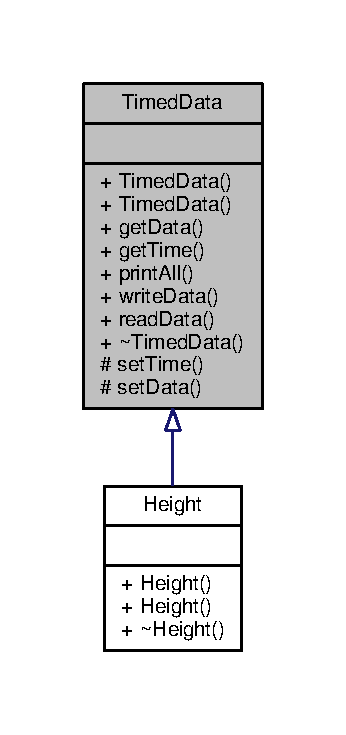
\includegraphics[width=166pt]{classTimedData__inherit__graph}
\end{center}
\end{figure}
\subsection*{Public Member Functions}
\begin{DoxyCompactItemize}
\item 
\hyperlink{classTimedData_abed3263e78c1a55e7ff5fe6a50185317}{Timed\+Data} ()
\item 
\hyperlink{classTimedData_a96f4b1aba52e95af687db6d71fa19bfa}{Timed\+Data} (float data, microseconds time)
\item 
float \hyperlink{classTimedData_aa8b1827a1b723de9ddd2582494927170}{get\+Data} ()
\item 
microseconds \hyperlink{classTimedData_a0012907b806867efc968db0d618213a6}{get\+Time} ()
\item 
\hypertarget{classTimedData_aaff93a393397a9dc1823652f8a0f89cc}{void \hyperlink{classTimedData_aaff93a393397a9dc1823652f8a0f89cc}{print\+All} ()}\label{classTimedData_aaff93a393397a9dc1823652f8a0f89cc}

\begin{DoxyCompactList}\small\item\em print contents of \hyperlink{classTimedData}{Timed\+Data} to console \end{DoxyCompactList}\item 
void \hyperlink{classTimedData_a6ae616a87f0f8ed004445b2fd6b1ba7d}{write\+Data} (string filename, \hyperlink{classTimedData}{Timed\+Data} $\ast$h)
\item 
void \hyperlink{classTimedData_a4b4ece4a2ab9c68e3fb0e2f1983819c5}{read\+Data} (string filename, \hyperlink{classTimedData}{Timed\+Data} $\ast$h)
\item 
\hyperlink{classTimedData_a9963efb752073782ab0cc4442cd41172}{$\sim$\+Timed\+Data} (void)
\end{DoxyCompactItemize}
\subsection*{Protected Member Functions}
\begin{DoxyCompactItemize}
\item 
void \hyperlink{classTimedData_a95d97c33cc4107ac10590aad5522f7a1}{set\+Time} (microseconds t)
\item 
void \hyperlink{classTimedData_aab7f26960dd570f86b8893352444411d}{set\+Data} (float d)
\end{DoxyCompactItemize}


\subsection{Detailed Description}
Store \hyperlink{classTimedData}{Timed\+Data} data and time-\/stamp 

\subsection{Constructor \& Destructor Documentation}
\hypertarget{classTimedData_abed3263e78c1a55e7ff5fe6a50185317}{\index{Timed\+Data@{Timed\+Data}!Timed\+Data@{Timed\+Data}}
\index{Timed\+Data@{Timed\+Data}!Timed\+Data@{Timed\+Data}}
\subsubsection[{Timed\+Data}]{\setlength{\rightskip}{0pt plus 5cm}Timed\+Data\+::\+Timed\+Data (
\begin{DoxyParamCaption}
{}
\end{DoxyParamCaption}
)}}\label{classTimedData_abed3263e78c1a55e7ff5fe6a50185317}
Construct an empty \hyperlink{classTimedData}{Timed\+Data} object \begin{DoxyPostcond}{Postcondition}
an empty \hyperlink{classTimedData}{Timed\+Data} object is created 
\end{DoxyPostcond}


Here is the call graph for this function\+:\nopagebreak
\begin{figure}[H]
\begin{center}
\leavevmode
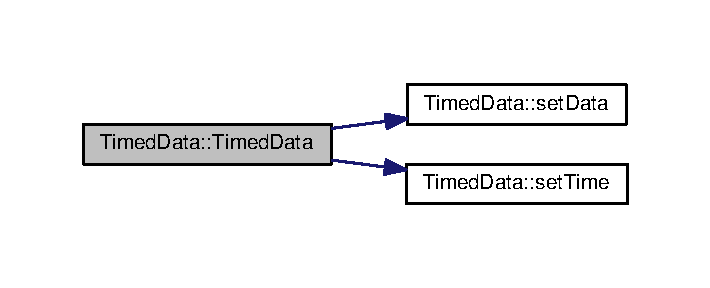
\includegraphics[width=341pt]{classTimedData_abed3263e78c1a55e7ff5fe6a50185317_cgraph}
\end{center}
\end{figure}


\hypertarget{classTimedData_a96f4b1aba52e95af687db6d71fa19bfa}{\index{Timed\+Data@{Timed\+Data}!Timed\+Data@{Timed\+Data}}
\index{Timed\+Data@{Timed\+Data}!Timed\+Data@{Timed\+Data}}
\subsubsection[{Timed\+Data}]{\setlength{\rightskip}{0pt plus 5cm}Timed\+Data\+::\+Timed\+Data (
\begin{DoxyParamCaption}
\item[{float}]{data, }
\item[{microseconds}]{time}
\end{DoxyParamCaption}
)}}\label{classTimedData_a96f4b1aba52e95af687db6d71fa19bfa}
Construct a \hyperlink{classTimedData}{Timed\+Data} object with provided parameters 
\begin{DoxyParams}[1]{Parameters}
\mbox{\tt in}  & {\em time} & the data was taken \\
\hline
\mbox{\tt in}  & {\em data} & any data \\
\hline
\end{DoxyParams}
\begin{DoxyPostcond}{Postcondition}
A \hyperlink{classTimedData}{Timed\+Data} object containing a \hyperlink{classTimedData}{Timed\+Data} reading and the corresponding time-\/stamp 
\end{DoxyPostcond}


Here is the call graph for this function\+:\nopagebreak
\begin{figure}[H]
\begin{center}
\leavevmode
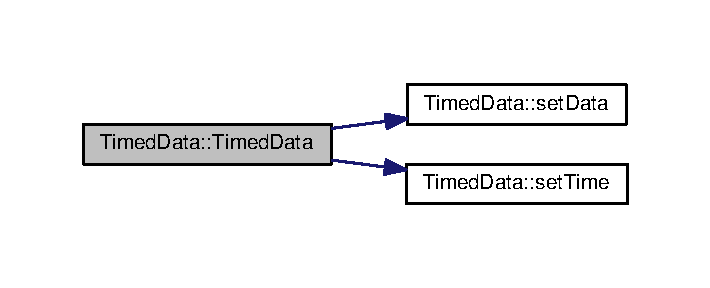
\includegraphics[width=341pt]{classTimedData_a96f4b1aba52e95af687db6d71fa19bfa_cgraph}
\end{center}
\end{figure}


\hypertarget{classTimedData_a9963efb752073782ab0cc4442cd41172}{\index{Timed\+Data@{Timed\+Data}!````~Timed\+Data@{$\sim$\+Timed\+Data}}
\index{````~Timed\+Data@{$\sim$\+Timed\+Data}!Timed\+Data@{Timed\+Data}}
\subsubsection[{$\sim$\+Timed\+Data}]{\setlength{\rightskip}{0pt plus 5cm}Timed\+Data\+::$\sim$\+Timed\+Data (
\begin{DoxyParamCaption}
\item[{void}]{}
\end{DoxyParamCaption}
)}}\label{classTimedData_a9963efb752073782ab0cc4442cd41172}
Destructor for \hyperlink{classTimedData}{Timed\+Data} object 

\subsection{Member Function Documentation}
\hypertarget{classTimedData_aa8b1827a1b723de9ddd2582494927170}{\index{Timed\+Data@{Timed\+Data}!get\+Data@{get\+Data}}
\index{get\+Data@{get\+Data}!Timed\+Data@{Timed\+Data}}
\subsubsection[{get\+Data}]{\setlength{\rightskip}{0pt plus 5cm}float Timed\+Data\+::get\+Data (
\begin{DoxyParamCaption}
{}
\end{DoxyParamCaption}
)}}\label{classTimedData_aa8b1827a1b723de9ddd2582494927170}
\begin{DoxyReturn}{Returns}
Data held in \hyperlink{classTimedData}{Timed\+Data} 
\end{DoxyReturn}
\hypertarget{classTimedData_a0012907b806867efc968db0d618213a6}{\index{Timed\+Data@{Timed\+Data}!get\+Time@{get\+Time}}
\index{get\+Time@{get\+Time}!Timed\+Data@{Timed\+Data}}
\subsubsection[{get\+Time}]{\setlength{\rightskip}{0pt plus 5cm}microseconds Timed\+Data\+::get\+Time (
\begin{DoxyParamCaption}
{}
\end{DoxyParamCaption}
)}}\label{classTimedData_a0012907b806867efc968db0d618213a6}
\begin{DoxyReturn}{Returns}
time of Data 
\end{DoxyReturn}
\hypertarget{classTimedData_a4b4ece4a2ab9c68e3fb0e2f1983819c5}{\index{Timed\+Data@{Timed\+Data}!read\+Data@{read\+Data}}
\index{read\+Data@{read\+Data}!Timed\+Data@{Timed\+Data}}
\subsubsection[{read\+Data}]{\setlength{\rightskip}{0pt plus 5cm}void Timed\+Data\+::read\+Data (
\begin{DoxyParamCaption}
\item[{string}]{filename, }
\item[{{\bf Timed\+Data} $\ast$}]{h}
\end{DoxyParamCaption}
)}}\label{classTimedData_a4b4ece4a2ab9c68e3fb0e2f1983819c5}
read \hyperlink{classTimedData}{Timed\+Data} object from file 
\begin{DoxyParams}[1]{Parameters}
\mbox{\tt in}  & {\em filename} & name of file to be read \\
\hline
\mbox{\tt in}  & {\em h} & pointer to the \hyperlink{classTimedData}{Timed\+Data} object being read \\
\hline
\end{DoxyParams}
\begin{DoxyPrecond}{Precondition}
A file containing at least one \hyperlink{classTimedData}{Timed\+Data} object stored in binary 

A \hyperlink{classTimedData}{Timed\+Data} object to store the data from file 
\end{DoxyPrecond}
\begin{DoxyPostcond}{Postcondition}
A \hyperlink{classTimedData}{Timed\+Data} object containing data from the file being read 
\end{DoxyPostcond}
\hypertarget{classTimedData_aab7f26960dd570f86b8893352444411d}{\index{Timed\+Data@{Timed\+Data}!set\+Data@{set\+Data}}
\index{set\+Data@{set\+Data}!Timed\+Data@{Timed\+Data}}
\subsubsection[{set\+Data}]{\setlength{\rightskip}{0pt plus 5cm}void Timed\+Data\+::set\+Data (
\begin{DoxyParamCaption}
\item[{float}]{d}
\end{DoxyParamCaption}
)\hspace{0.3cm}{\ttfamily [protected]}}}\label{classTimedData_aab7f26960dd570f86b8893352444411d}
set Data member 
\begin{DoxyParams}[1]{Parameters}
\mbox{\tt in}  & {\em d} & the data \\
\hline
\end{DoxyParams}
\begin{DoxyPostcond}{Postcondition}
the Data member is set 
\end{DoxyPostcond}
\hypertarget{classTimedData_a95d97c33cc4107ac10590aad5522f7a1}{\index{Timed\+Data@{Timed\+Data}!set\+Time@{set\+Time}}
\index{set\+Time@{set\+Time}!Timed\+Data@{Timed\+Data}}
\subsubsection[{set\+Time}]{\setlength{\rightskip}{0pt plus 5cm}void Timed\+Data\+::set\+Time (
\begin{DoxyParamCaption}
\item[{microseconds}]{t}
\end{DoxyParamCaption}
)\hspace{0.3cm}{\ttfamily [protected]}}}\label{classTimedData_a95d97c33cc4107ac10590aad5522f7a1}
set time member 
\begin{DoxyParams}[1]{Parameters}
\mbox{\tt in}  & {\em t} & the timestamp of the data \\
\hline
\end{DoxyParams}
\begin{DoxyPostcond}{Postcondition}
time member is set to t 
\end{DoxyPostcond}
\hypertarget{classTimedData_a6ae616a87f0f8ed004445b2fd6b1ba7d}{\index{Timed\+Data@{Timed\+Data}!write\+Data@{write\+Data}}
\index{write\+Data@{write\+Data}!Timed\+Data@{Timed\+Data}}
\subsubsection[{write\+Data}]{\setlength{\rightskip}{0pt plus 5cm}void Timed\+Data\+::write\+Data (
\begin{DoxyParamCaption}
\item[{string}]{filename, }
\item[{{\bf Timed\+Data} $\ast$}]{h}
\end{DoxyParamCaption}
)}}\label{classTimedData_a6ae616a87f0f8ed004445b2fd6b1ba7d}
Save \hyperlink{classTimedData}{Timed\+Data} object to file 
\begin{DoxyParams}[1]{Parameters}
\mbox{\tt in}  & {\em filename} & name of file to be written \\
\hline
\mbox{\tt in}  & {\em h} & pointer to the \hyperlink{classTimedData}{Timed\+Data} object being written \\
\hline
\end{DoxyParams}
\begin{DoxyPrecond}{Precondition}
An existing \hyperlink{classTimedData}{Timed\+Data} object 
\end{DoxyPrecond}
\begin{DoxyPostcond}{Postcondition}
Object is saved to a binary file on disk 
\end{DoxyPostcond}


The documentation for this class was generated from the following files\+:\begin{DoxyCompactItemize}
\item 
Timed\+Data.\+hpp\item 
Timed\+Data.\+cpp\end{DoxyCompactItemize}

\hypertarget{classVerticalData}{\section{Vertical\+Data Class Reference}
\label{classVerticalData}\index{Vertical\+Data@{Vertical\+Data}}
}


Store two \hyperlink{classHeight}{Height} objects and calculate vertical velocity.  




{\ttfamily \#include $<$Vertical\+Data.\+hpp$>$}

\subsection*{Public Member Functions}
\begin{DoxyCompactItemize}
\item 
void \hyperlink{classVerticalData_a50b355687804c6d9b03e90bce2a3095e}{store\+Height} (\hyperlink{classHeight}{Height} \&ht)
\begin{DoxyCompactList}\small\item\em Store height object. \end{DoxyCompactList}\item 
void \hyperlink{classVerticalData_aef83569982446e500bd333c8a85b6f3a}{place\+Height} (float height, microseconds time)
\begin{DoxyCompactList}\small\item\em create \hyperlink{classHeight}{Height} object and place in queue \end{DoxyCompactList}\item 
float \hyperlink{classVerticalData_a6de4f8e0da7c7b31072c4a078b62d063}{get\+Velocity} ()
\item 
void \hyperlink{classVerticalData_a33097c244e4c8b4693aaecb60942fe41}{set\+Velocity} (float vel)
\item 
\hypertarget{classVerticalData_aa0e879c93866136cdfa2f8130b5eac17}{void \hyperlink{classVerticalData_aa0e879c93866136cdfa2f8130b5eac17}{print\+All} ()}\label{classVerticalData_aa0e879c93866136cdfa2f8130b5eac17}

\begin{DoxyCompactList}\small\item\em Print contents of \hyperlink{classVerticalData}{Vertical\+Data} object. \end{DoxyCompactList}\end{DoxyCompactItemize}
\subsection*{Protected Member Functions}
\begin{DoxyCompactItemize}
\item 
\hypertarget{classVerticalData_a6399ba01c41d1468f098e5efd88a1032}{void \hyperlink{classVerticalData_a6399ba01c41d1468f098e5efd88a1032}{calculate\+Velocity} ()}\label{classVerticalData_a6399ba01c41d1468f098e5efd88a1032}

\begin{DoxyCompactList}\small\item\em Calculate the vertical velocity. \end{DoxyCompactList}\end{DoxyCompactItemize}


\subsection{Detailed Description}
Store two \hyperlink{classHeight}{Height} objects and calculate vertical velocity. 

\subsection{Member Function Documentation}
\hypertarget{classVerticalData_a6de4f8e0da7c7b31072c4a078b62d063}{\index{Vertical\+Data@{Vertical\+Data}!get\+Velocity@{get\+Velocity}}
\index{get\+Velocity@{get\+Velocity}!Vertical\+Data@{Vertical\+Data}}
\subsubsection[{get\+Velocity}]{\setlength{\rightskip}{0pt plus 5cm}float Vertical\+Data\+::get\+Velocity (
\begin{DoxyParamCaption}
{}
\end{DoxyParamCaption}
)}}\label{classVerticalData_a6de4f8e0da7c7b31072c4a078b62d063}
\begin{DoxyReturn}{Returns}
vertical velocity 
\end{DoxyReturn}
\hypertarget{classVerticalData_aef83569982446e500bd333c8a85b6f3a}{\index{Vertical\+Data@{Vertical\+Data}!place\+Height@{place\+Height}}
\index{place\+Height@{place\+Height}!Vertical\+Data@{Vertical\+Data}}
\subsubsection[{place\+Height}]{\setlength{\rightskip}{0pt plus 5cm}void Vertical\+Data\+::place\+Height (
\begin{DoxyParamCaption}
\item[{float}]{height, }
\item[{microseconds}]{time}
\end{DoxyParamCaption}
)}}\label{classVerticalData_aef83569982446e500bd333c8a85b6f3a}


create \hyperlink{classHeight}{Height} object and place in queue 


\begin{DoxyParams}[1]{Parameters}
\mbox{\tt in}  & {\em height} & height of U\+A\+V in meters \\
\hline
\mbox{\tt in}  & {\em time} & timestamp of height in microseconds \\
\hline
\end{DoxyParams}
\hypertarget{classVerticalData_a33097c244e4c8b4693aaecb60942fe41}{\index{Vertical\+Data@{Vertical\+Data}!set\+Velocity@{set\+Velocity}}
\index{set\+Velocity@{set\+Velocity}!Vertical\+Data@{Vertical\+Data}}
\subsubsection[{set\+Velocity}]{\setlength{\rightskip}{0pt plus 5cm}void Vertical\+Data\+::set\+Velocity (
\begin{DoxyParamCaption}
\item[{float}]{vel}
\end{DoxyParamCaption}
)}}\label{classVerticalData_a33097c244e4c8b4693aaecb60942fe41}

\begin{DoxyParams}{Parameters}
{\em vel} & the velocity of the U\+A\+V in m/s \\
\hline
\end{DoxyParams}
\hypertarget{classVerticalData_a50b355687804c6d9b03e90bce2a3095e}{\index{Vertical\+Data@{Vertical\+Data}!store\+Height@{store\+Height}}
\index{store\+Height@{store\+Height}!Vertical\+Data@{Vertical\+Data}}
\subsubsection[{store\+Height}]{\setlength{\rightskip}{0pt plus 5cm}void Vertical\+Data\+::store\+Height (
\begin{DoxyParamCaption}
\item[{{\bf Height} \&}]{ht}
\end{DoxyParamCaption}
)}}\label{classVerticalData_a50b355687804c6d9b03e90bce2a3095e}


Store height object. 


\begin{DoxyParams}[1]{Parameters}
\mbox{\tt in}  & {\em ht} & the height of the U\+A\+V in meters \\
\hline
\end{DoxyParams}


The documentation for this class was generated from the following files\+:\begin{DoxyCompactItemize}
\item 
Vertical\+Data.\+hpp\item 
Vertical\+Data.\+cpp\end{DoxyCompactItemize}

\chapter{File Documentation}
\hypertarget{mega__sensor_8h}{\section{mega\+\_\+sensor.\+h File Reference}
\label{mega__sensor_8h}\index{mega\+\_\+sensor.\+h@{mega\+\_\+sensor.\+h}}
}


get sensor data  


{\ttfamily \#include $<$unistd.\+h$>$}\\*
{\ttfamily \#include $<$math.\+h$>$}\\*
{\ttfamily \#include $<$stdio.\+h$>$}\\*
{\ttfamily \#include $<$signal.\+h$>$}\\*
{\ttfamily \#include $<$stdlib.\+h$>$}\\*
{\ttfamily \#include $<$fcntl.\+h$>$}\\*
{\ttfamily \#include $<$string.\+h$>$}\\*
{\ttfamily \#include $<$time.\+h$>$}\\*
{\ttfamily \#include $<$wiring\+Pi.\+h$>$}\\*
{\ttfamily \#include \char`\"{}../include/lidar\+Lite.\+h\char`\"{}}\\*
{\ttfamily \#include \char`\"{}../includes/sensor.\+h\char`\"{}}\\*
{\ttfamily \#include \char`\"{}../includes/output.\+h\char`\"{}}\\*
{\ttfamily \#include \char`\"{}../includes/bmp180.\+h\char`\"{}}\\*
\subsection*{Functions}
\begin{DoxyCompactItemize}
\item 
void \hyperlink{mega__sensor_8h_a24ad36b35639619a3489817e76a1a860}{M\+E\+G\+A\+\_\+\+S\+E\+N\+S\+O\+R} (float $\ast$g\+\_\+x, float $\ast$g\+\_\+y, float $\ast$a\+\_\+x, float $\ast$a\+\_\+y, float $\ast$t, long $\ast$p, int $\ast$l, float $\ast$l\+\_\+c, long $\ast$b\+\_\+c, float $\ast$h, int fd)
\end{DoxyCompactItemize}


\subsection{Detailed Description}
get sensor data 

\begin{DoxyAuthor}{Author}
Luke Protz 
\end{DoxyAuthor}


\subsection{Function Documentation}
\hypertarget{mega__sensor_8h_a24ad36b35639619a3489817e76a1a860}{\index{mega\+\_\+sensor.\+h@{mega\+\_\+sensor.\+h}!M\+E\+G\+A\+\_\+\+S\+E\+N\+S\+O\+R@{M\+E\+G\+A\+\_\+\+S\+E\+N\+S\+O\+R}}
\index{M\+E\+G\+A\+\_\+\+S\+E\+N\+S\+O\+R@{M\+E\+G\+A\+\_\+\+S\+E\+N\+S\+O\+R}!mega\+\_\+sensor.\+h@{mega\+\_\+sensor.\+h}}
\subsubsection[{M\+E\+G\+A\+\_\+\+S\+E\+N\+S\+O\+R}]{\setlength{\rightskip}{0pt plus 5cm}void M\+E\+G\+A\+\_\+\+S\+E\+N\+S\+O\+R (
\begin{DoxyParamCaption}
\item[{float $\ast$}]{g\+\_\+x, }
\item[{float $\ast$}]{g\+\_\+y, }
\item[{float $\ast$}]{a\+\_\+x, }
\item[{float $\ast$}]{a\+\_\+y, }
\item[{float $\ast$}]{t, }
\item[{long $\ast$}]{p, }
\item[{int $\ast$}]{l, }
\item[{float $\ast$}]{l\+\_\+c, }
\item[{long $\ast$}]{b\+\_\+c, }
\item[{float $\ast$}]{h, }
\item[{int}]{fd}
\end{DoxyParamCaption}
)}}\label{mega__sensor_8h_a24ad36b35639619a3489817e76a1a860}
\begin{DoxyPrecond}{Precondition}
The Lidar is initialized 

The I\+M\+U is initialized 
\end{DoxyPrecond}

\begin{DoxyParams}[1]{Parameters}
\mbox{\tt out}  & {\em g\+\_\+x} & acceleration in the x direction in \\
\hline
\mbox{\tt out}  & {\em g\+\_\+y} & acceleration in the y direction \\
\hline
\mbox{\tt out}  & {\em a\+\_\+x} & \\
\hline
\mbox{\tt out}  & {\em a\+\_\+y} & \\
\hline
\mbox{\tt out}  & {\em t} & \\
\hline
\mbox{\tt out}  & {\em p} & \\
\hline
\mbox{\tt out}  & {\em l} & \\
\hline
\mbox{\tt out}  & {\em l} & \\
\hline
\mbox{\tt out}  & {\em l\+\_\+c} & \\
\hline
\mbox{\tt out}  & {\em b\+\_\+c} & \\
\hline
\mbox{\tt out}  & {\em fd} & \\
\hline
\mbox{\tt out}  & {\em } & post \\
\hline
\end{DoxyParams}

\hypertarget{velocityCalculate_8hpp}{\section{velocity\+Calculate.\+hpp File Reference}
\label{velocityCalculate_8hpp}\index{velocity\+Calculate.\+hpp@{velocity\+Calculate.\+hpp}}
}


Calculate the Horizontal Velocity of a U\+A\+V.  


{\ttfamily \#include $<$opencv2/video/tracking.\+hpp$>$}\\*
{\ttfamily \#include $<$opencv2/imgproc/imgproc.\+hpp$>$}\\*
{\ttfamily \#include $<$opencv2/highgui/highgui.\+hpp$>$}\\*
{\ttfamily \#include $<$iostream$>$}\\*
{\ttfamily \#include $<$ctype.\+h$>$}\\*
{\ttfamily \#include $<$iomanip$>$}\\*
{\ttfamily \#include $<$random$>$}\\*
\subsection*{Functions}
\begin{DoxyCompactItemize}
\item 
void \hyperlink{velocityCalculate_8hpp_a118131c72f75d5aca6ad7631de0eda64}{four\+Pixel\+Average} (Input\+Array img\+Full, Output\+Array img\+Reduced)
\begin{DoxyCompactList}\small\item\em average four pixels \end{DoxyCompactList}\item 
float \hyperlink{velocityCalculate_8hpp_accfa483afa5017fd06388c4de09416b4}{entropy} (Mat seq, Size size, int index)
\begin{DoxyCompactList}\small\item\em calculate the entropy of an image \end{DoxyCompactList}\item 
Mat \hyperlink{velocityCalculate_8hpp_afe324ff9e0136d24643fb5d2c49e6d89}{my\+Entropy} (Mat seq, int hist\+Size)
\begin{DoxyCompactList}\small\item\em calculates relative occurrence of different symbols within given input sequence using histogram \end{DoxyCompactList}\item 
void \hyperlink{velocityCalculate_8hpp_aeeb54087a0d0b7c6418fccb0308e1a34}{calculate\+A\+E\+A\+O} (Mat prev\+Gray, Mat next\+Gray, double camera\+Elevation, int frame\+Rate, double pitch, double roll, double w\+Pitch, double w\+Roll, double \&Vx, double \&Vy, double Vz, double \&speed, double \&direction)
\begin{DoxyCompactList}\small\item\em Calculates velocity in the x and y directions,speed and direction of an unmanned aerial vehicle(\+U\+A\+V). \end{DoxyCompactList}\end{DoxyCompactItemize}


\subsection{Detailed Description}
Calculate the Horizontal Velocity of a U\+A\+V. 

\begin{DoxyDate}{Date}
Mar 26, 2016 
\end{DoxyDate}
\begin{DoxyAuthor}{Author}
Lance Pitka 

Devon Haubold 
\end{DoxyAuthor}


\subsection{Function Documentation}
\hypertarget{velocityCalculate_8hpp_aeeb54087a0d0b7c6418fccb0308e1a34}{\index{velocity\+Calculate.\+hpp@{velocity\+Calculate.\+hpp}!calculate\+A\+E\+A\+O@{calculate\+A\+E\+A\+O}}
\index{calculate\+A\+E\+A\+O@{calculate\+A\+E\+A\+O}!velocity\+Calculate.\+hpp@{velocity\+Calculate.\+hpp}}
\subsubsection[{calculate\+A\+E\+A\+O}]{\setlength{\rightskip}{0pt plus 5cm}void calculate\+A\+E\+A\+O (
\begin{DoxyParamCaption}
\item[{Mat}]{prev\+Gray, }
\item[{Mat}]{next\+Gray, }
\item[{double}]{camera\+Elevation, }
\item[{int}]{frame\+Rate, }
\item[{double}]{pitch, }
\item[{double}]{roll, }
\item[{double}]{w\+Pitch, }
\item[{double}]{w\+Roll, }
\item[{double \&}]{Vx, }
\item[{double \&}]{Vy, }
\item[{double}]{Vz, }
\item[{double \&}]{speed, }
\item[{double \&}]{direction}
\end{DoxyParamCaption}
)}}\label{velocityCalculate_8hpp_aeeb54087a0d0b7c6418fccb0308e1a34}


Calculates velocity in the x and y directions,speed and direction of an unmanned aerial vehicle(\+U\+A\+V). 

Calculates confidence in calculations \begin{DoxyPrecond}{Precondition}
Two images, prev\+Gray and next\+Gray, taken successively at a specified frame rate 

Pitch, \hyperlink{classHeight}{Height}, Vz, Roll, change in pitch, change in Roll, at the time the images are captured 

Vx, Vy, speed and Direction are declared 
\end{DoxyPrecond}

\begin{DoxyParams}[1]{Parameters}
\mbox{\tt in}  & {\em prev\+Gray} & the first single channel 8bit image \\
\hline
\mbox{\tt in}  & {\em next\+Gray} & the second single channel 8bit image \\
\hline
\mbox{\tt in}  & {\em camera\+Elevation} & the distance of the U\+A\+V from the ground \\
\hline
\mbox{\tt in}  & {\em frame\+Rate} & rate at which the images are being captured in fps \\
\hline
\mbox{\tt in}  & {\em pitch} & the pitch of the U\+A\+V in radians \\
\hline
\mbox{\tt in}  & {\em roll} & the roll of the U\+A\+V in radians \\
\hline
\mbox{\tt in}  & {\em w\+Pitch} & the U\+A\+V angular pitch velocity in radians/sec \\
\hline
\mbox{\tt in}  & {\em w\+Roll} & the U\+A\+V angular roll velocity in radians/sec \\
\hline
\mbox{\tt out}  & {\em Vx} & U\+A\+V velocity in the x direction \\
\hline
\mbox{\tt out}  & {\em Vy} & U\+A\+V velocity in the y direction \\
\hline
\mbox{\tt in,out}  & {\em Vz} & U\+A\+V Velocity in the z direction (vertical velocity) in m/s \\
\hline
\mbox{\tt out}  & {\em speed} & the speed of U\+A\+V in m/s \\
\hline
\mbox{\tt out}  & {\em direction} & direction of the U\+A\+V in radians relative to itself. \\
\hline
\end{DoxyParams}
\begin{DoxyPostcond}{Postcondition}
Vx contains the most recent velocity in the x direction 

Vy contains the most recent Velocity in the y direction 

speed contains the most recent speed 

direction contains the most recent direction 
\end{DoxyPostcond}


Here is the call graph for this function\+:\nopagebreak
\begin{figure}[H]
\begin{center}
\leavevmode
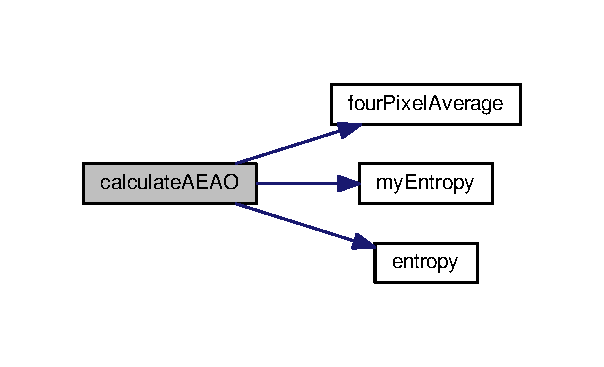
\includegraphics[width=290pt]{velocityCalculate_8hpp_aeeb54087a0d0b7c6418fccb0308e1a34_cgraph}
\end{center}
\end{figure}


\hypertarget{velocityCalculate_8hpp_accfa483afa5017fd06388c4de09416b4}{\index{velocity\+Calculate.\+hpp@{velocity\+Calculate.\+hpp}!entropy@{entropy}}
\index{entropy@{entropy}!velocity\+Calculate.\+hpp@{velocity\+Calculate.\+hpp}}
\subsubsection[{entropy}]{\setlength{\rightskip}{0pt plus 5cm}float entropy (
\begin{DoxyParamCaption}
\item[{Mat}]{seq, }
\item[{Size}]{size, }
\item[{int}]{index}
\end{DoxyParamCaption}
)}}\label{velocityCalculate_8hpp_accfa483afa5017fd06388c4de09416b4}


calculate the entropy of an image 


\begin{DoxyParams}[1]{Parameters}
\mbox{\tt in}  & {\em seq} & a single channel 8 bit image \\
\hline
\mbox{\tt in}  & {\em size} & dimensions of image \\
\hline
\mbox{\tt in}  & {\em index} & pixel location in image \\
\hline
\end{DoxyParams}
\begin{DoxyReturn}{Returns}
the entropy of the image at index 
\end{DoxyReturn}
\hypertarget{velocityCalculate_8hpp_a118131c72f75d5aca6ad7631de0eda64}{\index{velocity\+Calculate.\+hpp@{velocity\+Calculate.\+hpp}!four\+Pixel\+Average@{four\+Pixel\+Average}}
\index{four\+Pixel\+Average@{four\+Pixel\+Average}!velocity\+Calculate.\+hpp@{velocity\+Calculate.\+hpp}}
\subsubsection[{four\+Pixel\+Average}]{\setlength{\rightskip}{0pt plus 5cm}void four\+Pixel\+Average (
\begin{DoxyParamCaption}
\item[{Input\+Array}]{img\+Full, }
\item[{Output\+Array}]{img\+Reduced}
\end{DoxyParamCaption}
)}}\label{velocityCalculate_8hpp_a118131c72f75d5aca6ad7631de0eda64}


average four pixels 


\begin{DoxyParams}[1]{Parameters}
\mbox{\tt in}  & {\em img\+Full} & the image to be averaged \\
\hline
\mbox{\tt out}  & {\em img\+Reduced} & an averaged image \\
\hline
\end{DoxyParams}
\hypertarget{velocityCalculate_8hpp_afe324ff9e0136d24643fb5d2c49e6d89}{\index{velocity\+Calculate.\+hpp@{velocity\+Calculate.\+hpp}!my\+Entropy@{my\+Entropy}}
\index{my\+Entropy@{my\+Entropy}!velocity\+Calculate.\+hpp@{velocity\+Calculate.\+hpp}}
\subsubsection[{my\+Entropy}]{\setlength{\rightskip}{0pt plus 5cm}Mat my\+Entropy (
\begin{DoxyParamCaption}
\item[{Mat}]{seq, }
\item[{int}]{hist\+Size}
\end{DoxyParamCaption}
)}}\label{velocityCalculate_8hpp_afe324ff9e0136d24643fb5d2c49e6d89}


calculates relative occurrence of different symbols within given input sequence using histogram 


\begin{DoxyParams}[1]{Parameters}
\mbox{\tt in}  & {\em seq} & a single channel 8 bit image \\
\hline
\mbox{\tt in}  & {\em hist\+Size} & size of the histogram \\
\hline
\end{DoxyParams}
\begin{DoxyReturn}{Returns}
histogram showing occurence of symbols in a sequence 
\end{DoxyReturn}
Compute the histograms\+: 
\hypertarget{velocityTracking_8cpp}{\section{velocity\+Tracking.\+cpp File Reference}
\label{velocityTracking_8cpp}\index{velocity\+Tracking.\+cpp@{velocity\+Tracking.\+cpp}}
}


The main program, stores data and calculates velocities.  


{\ttfamily \#include \char`\"{}../includes/\+Height.\+hpp\char`\"{}}\\*
{\ttfamily \#include \char`\"{}../includes/\+Vertical\+Data.\+hpp\char`\"{}}\\*
{\ttfamily \#include \char`\"{}../includes/velocity\+Calculate.\+hpp\char`\"{}}\\*
{\ttfamily \#include \char`\"{}../includes/output.\+h\char`\"{}}\\*
{\ttfamily \#include \char`\"{}../includes/sensor.\+h\char`\"{}}\\*
{\ttfamily \#include \char`\"{}../includes/bmp180.\+h\char`\"{}}\\*
{\ttfamily \#include \char`\"{}../includes/lidar\+Lite.\+h\char`\"{}}\\*
{\ttfamily \#include \char`\"{}../includes/mega\+\_\+sensor.\+h\char`\"{}}\\*
{\ttfamily \#include $<$iostream$>$}\\*
{\ttfamily \#include $<$cstdlib$>$}\\*
{\ttfamily \#include $<$thread$>$}\\*
{\ttfamily \#include $<$chrono$>$}\\*
{\ttfamily \#include $<$ctime$>$}\\*
{\ttfamily \#include $<$opencv2/highgui/highgui.\+hpp$>$}\\*
{\ttfamily \#include $<$raspicam/raspicam\+\_\+cv.\+h$>$}\\*
\subsection*{Macros}
\begin{DoxyCompactItemize}
\item 
\#define \hyperlink{velocityTracking_8cpp_ae2f99e05f64d0383aee9bd75a52c4fbb}{F\+R\+A\+M\+E\+\_\+\+R\+A\+T\+E}~90
\end{DoxyCompactItemize}
\subsection*{Functions}
\begin{DoxyCompactItemize}
\item 
void \hyperlink{velocityTracking_8cpp_a339b674fe2736f27352f0615792ba220}{initialize\+Camera} (raspicam\+::\+Raspi\+Cam\+\_\+\+Cv \&Camera)
\item 
void \hyperlink{velocityTracking_8cpp_a6893ce6a000489582c4754d3e929faf2}{two\+Image\+Capture} (Mat \&image\+\_\+1, Mat \&image\+\_\+2, bool \&exit\+\_\+flag, bool \&ready\+\_\+flag, bool \&wait\+\_\+flag)
\begin{DoxyCompactList}\small\item\em capture two consecutive images at 90 frames per second, loops until exit\+\_\+flag is true \end{DoxyCompactList}\item 
void \hyperlink{velocityTracking_8cpp_a420d1601b90eadda1b8a5a0552f1991c}{height\+Reporting} (\hyperlink{classVerticalData}{Vertical\+Data} \&vert\+Data\+Ref, bool \&exit\+\_\+flag, int lidar)
\item 
int \hyperlink{velocityTracking_8cpp_a0ddf1224851353fc92bfbff6f499fa97}{main} (int argc, char $\ast$argv\mbox{[}$\,$\mbox{]})
\end{DoxyCompactItemize}


\subsection{Detailed Description}
The main program, stores data and calculates velocities. 

\begin{DoxyDate}{Date}
Mar 21, 2016 
\end{DoxyDate}
\begin{DoxyAuthor}{Author}
\+: Devon Haubold 
\end{DoxyAuthor}


\subsection{Macro Definition Documentation}
\hypertarget{velocityTracking_8cpp_ae2f99e05f64d0383aee9bd75a52c4fbb}{\index{velocity\+Tracking.\+cpp@{velocity\+Tracking.\+cpp}!F\+R\+A\+M\+E\+\_\+\+R\+A\+T\+E@{F\+R\+A\+M\+E\+\_\+\+R\+A\+T\+E}}
\index{F\+R\+A\+M\+E\+\_\+\+R\+A\+T\+E@{F\+R\+A\+M\+E\+\_\+\+R\+A\+T\+E}!velocity\+Tracking.\+cpp@{velocity\+Tracking.\+cpp}}
\subsubsection[{F\+R\+A\+M\+E\+\_\+\+R\+A\+T\+E}]{\setlength{\rightskip}{0pt plus 5cm}\#define F\+R\+A\+M\+E\+\_\+\+R\+A\+T\+E~90}}\label{velocityTracking_8cpp_ae2f99e05f64d0383aee9bd75a52c4fbb}
The frame rate that the camera is set at 

\subsection{Function Documentation}
\hypertarget{velocityTracking_8cpp_a420d1601b90eadda1b8a5a0552f1991c}{\index{velocity\+Tracking.\+cpp@{velocity\+Tracking.\+cpp}!height\+Reporting@{height\+Reporting}}
\index{height\+Reporting@{height\+Reporting}!velocity\+Tracking.\+cpp@{velocity\+Tracking.\+cpp}}
\subsubsection[{height\+Reporting}]{\setlength{\rightskip}{0pt plus 5cm}void height\+Reporting (
\begin{DoxyParamCaption}
\item[{{\bf Vertical\+Data} \&}]{vert\+Data\+Ref, }
\item[{bool \&}]{exit\+\_\+flag, }
\item[{int}]{lidar}
\end{DoxyParamCaption}
)}}\label{velocityTracking_8cpp_a420d1601b90eadda1b8a5a0552f1991c}
Get height data continuosly, calculate velocity \begin{DoxyPrecond}{Precondition}
a thread has been created and id assigned 

the sensors have been initialized and are accessible 
\end{DoxyPrecond}

\begin{DoxyParams}[1]{Parameters}
\mbox{\tt in}  & {\em vert\+Data\+Ref} & holds height data and calculates vertical velocity \\
\hline
\mbox{\tt in}  & {\em exit\+\_\+flag} & flag to alert thread to exit \\
\hline
\mbox{\tt in}  & {\em lidar} & equals 1 if lidar is initialized \\
\hline
\end{DoxyParams}


Here is the call graph for this function\+:
\nopagebreak
\begin{figure}[H]
\begin{center}
\leavevmode
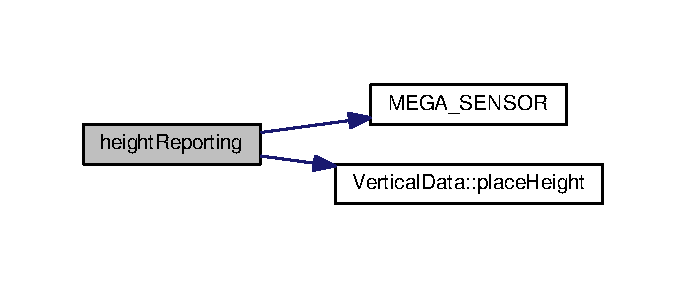
\includegraphics[width=350pt]{velocityTracking_8cpp_a420d1601b90eadda1b8a5a0552f1991c_cgraph}
\end{center}
\end{figure}


\hypertarget{velocityTracking_8cpp_a339b674fe2736f27352f0615792ba220}{\index{velocity\+Tracking.\+cpp@{velocity\+Tracking.\+cpp}!initialize\+Camera@{initialize\+Camera}}
\index{initialize\+Camera@{initialize\+Camera}!velocity\+Tracking.\+cpp@{velocity\+Tracking.\+cpp}}
\subsubsection[{initialize\+Camera}]{\setlength{\rightskip}{0pt plus 5cm}void initialize\+Camera (
\begin{DoxyParamCaption}
\item[{raspicam\+::\+Raspi\+Cam\+\_\+\+Cv \&}]{Camera}
\end{DoxyParamCaption}
)}}\label{velocityTracking_8cpp_a339b674fe2736f27352f0615792ba220}
\begin{DoxyPostcond}{Postcondition}
camera image format set to single channel 8 bit 

gain set to maximum value 
\end{DoxyPostcond}

\begin{DoxyParams}[1]{Parameters}
\mbox{\tt in,out}  & {\em Camera} & the camera interface \\
\hline
\end{DoxyParams}
\hypertarget{velocityTracking_8cpp_a0ddf1224851353fc92bfbff6f499fa97}{\index{velocity\+Tracking.\+cpp@{velocity\+Tracking.\+cpp}!main@{main}}
\index{main@{main}!velocity\+Tracking.\+cpp@{velocity\+Tracking.\+cpp}}
\subsubsection[{main}]{\setlength{\rightskip}{0pt plus 5cm}int main (
\begin{DoxyParamCaption}
\item[{int}]{argc, }
\item[{char $\ast$}]{argv\mbox{[}$\,$\mbox{]}}
\end{DoxyParamCaption}
)}}\label{velocityTracking_8cpp_a0ddf1224851353fc92bfbff6f499fa97}
Declares input/output variables for sensor data Declares variables for calculated values Spawns threads using height\+Reporting and two\+Image\+Capture Calls velocity\+Calculate with sensor data and calculated value variables $<$ equals 1 if lidar initialized

wait until 1s has passed to get velocity every second 

Here is the call graph for this function\+:
\nopagebreak
\begin{figure}[H]
\begin{center}
\leavevmode
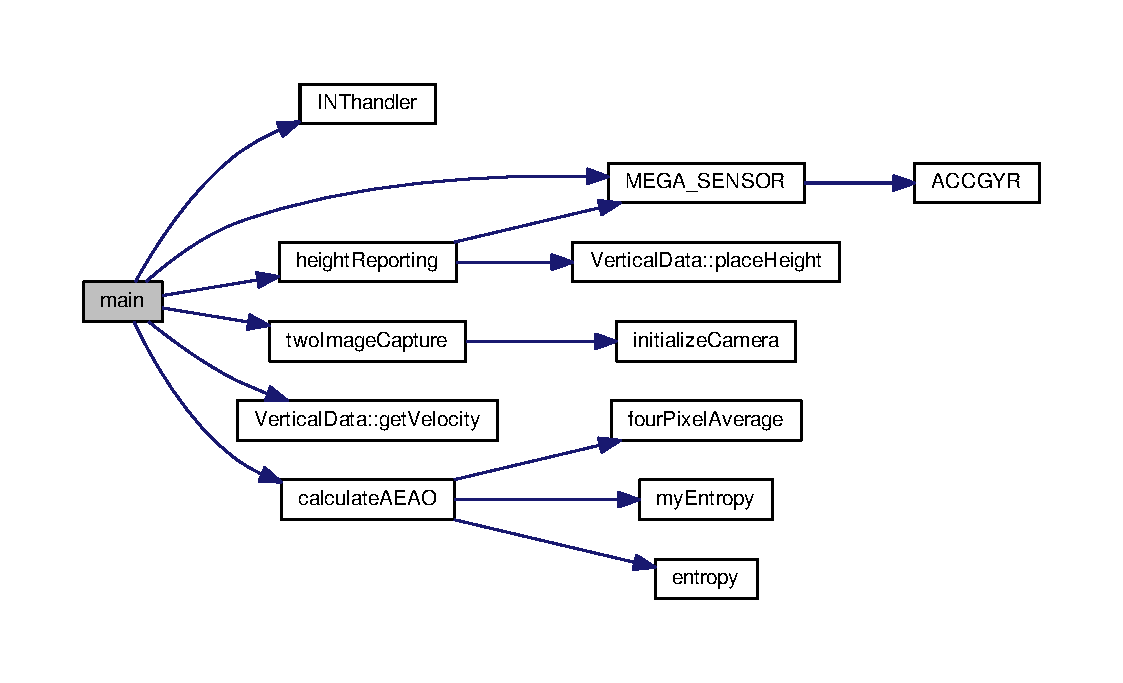
\includegraphics[width=350pt]{velocityTracking_8cpp_a0ddf1224851353fc92bfbff6f499fa97_cgraph}
\end{center}
\end{figure}


\hypertarget{velocityTracking_8cpp_a6893ce6a000489582c4754d3e929faf2}{\index{velocity\+Tracking.\+cpp@{velocity\+Tracking.\+cpp}!two\+Image\+Capture@{two\+Image\+Capture}}
\index{two\+Image\+Capture@{two\+Image\+Capture}!velocity\+Tracking.\+cpp@{velocity\+Tracking.\+cpp}}
\subsubsection[{two\+Image\+Capture}]{\setlength{\rightskip}{0pt plus 5cm}void two\+Image\+Capture (
\begin{DoxyParamCaption}
\item[{Mat \&}]{image\+\_\+1, }
\item[{Mat \&}]{image\+\_\+2, }
\item[{bool \&}]{exit\+\_\+flag, }
\item[{bool \&}]{ready\+\_\+flag, }
\item[{bool \&}]{wait\+\_\+flag}
\end{DoxyParamCaption}
)}}\label{velocityTracking_8cpp_a6893ce6a000489582c4754d3e929faf2}


capture two consecutive images at 90 frames per second, loops until exit\+\_\+flag is true 

\begin{DoxyPrecond}{Precondition}
a thread has been created and id assigned 
\end{DoxyPrecond}

\begin{DoxyParams}[1]{Parameters}
\mbox{\tt in,out}  & {\em image\+\_\+1} & the first image to be captured \\
\hline
\mbox{\tt in,out}  & {\em image\+\_\+2} & the second image to be captured \\
\hline
\mbox{\tt in}  & {\em exit\+\_\+flag} & flag to alert thread to exit \\
\hline
\mbox{\tt in,out}  & {\em ready\+\_\+flag} & to alert two images have been captured \\
\hline
\mbox{\tt in,out}  & {\em wait\+\_\+flag} & flag to alert images are being used \\
\hline
\end{DoxyParams}


Here is the call graph for this function\+:\nopagebreak
\begin{figure}[H]
\begin{center}
\leavevmode
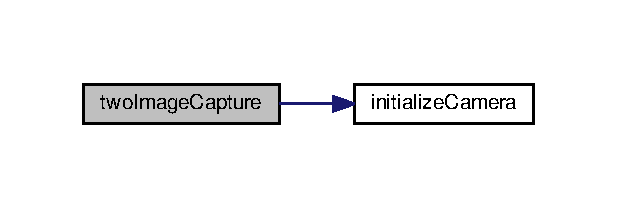
\includegraphics[width=296pt]{velocityTracking_8cpp_a6893ce6a000489582c4754d3e929faf2_cgraph}
\end{center}
\end{figure}



%--- End generated contents ---

% Index
\newpage
\phantomsection
\addcontentsline{toc}{chapter}{Index}
\printindex

\end{document}
